\section{Auxiliary Optics}
\subsection{Current State of the Art}
\subsubsection{Input optics}
\paragraph{Introduction}
In all the ground-based laser-interferometric gravitational wave detectors, the light which is injected into the main interferometer comes from high power lasers operating at 1064nm, with powers which could exceed 100 W (maximum 200W). Their frequency stability in the detection frequency band (10Hz-10kHz) is what you can find as the best in the world. Similarly, the relative intensity noise (RIN) of the laser beam is at the state of the art in laser power stabilization (2.10$^{-9}$/$\sqrt(Hz)$). Their spatial eigenmode is very close to an ideal Gaussian mode. In a first paragraph, we will give an overview of the function carried out by the Input optics.

\paragraph {Overview}

The Input Optics is the interface between the laser system and the Interferometer. It is also part of the Pre-stabilized laser. The whole system delivers a beam at the interferometer input port with the required power, geometrical shape, frequency and angular stability. An Electro Optic Modulation (EOM) system is providing the RF modulations needed for control and sensing purposes. The Input Mode Cleaner (IMC) cavity geometrically cleans the beam and reduces its amplitude and lateral fluctuation. The resonant IMC in conjunction with a reference cavity (RFC) are used to stabilize the laser frequency.
After the IMC some photodetectors provide the signal for intensity stabilization of the laser. An in-vacuum Faraday isolator prevents the light reflected by the interferometer goes back to the laser system and allows a simple extraction of this reflected beam. Finally, a mode matching telescope is used to properly match the beam on the Interferometer.

\paragraph {Wavelength and power handling}
In the first and second generation of GW detectors based on laser interferometers, the working wavelength is 1064nm which is produced by Nd:YAG solid state lasers. The power of the laser source in the first generation was of the order of a few tens of Watts which became a few hundred of Watts for the second generation. Up to now the detectors have been operated at a maximum of 50Watts injected in the interferometer but the plan is to reach 125Watts in the later developments of this generation. Due to the high power densities in the optical components such as the EOM system and the Faraday isolator, those devices has been specially developed for the Gravitational Wave detectors. 

\paragraph {Electro optic modulation system}
State of the art of the EOMs currently used will be given here.

\paragraph {Faraday isolators}
State of the art of the FIs currently used will be given here.

\paragraph {Input mode cleaner}
State of the art of the IMC cavities currently used will be given here.
Why Geo uses 2 IMCs?

\begin{table}[htp]
\begin{tabular}{@{}l c c c c c@{}}
Parameter & LIGO & Virgo & GEO & &Kagra\\
       &  &   &  IMC1  & IMC2 &  \\
\hline
Optical cavity length & 32.945 m & 286.845 m & 8 m & 8.1 m & 53.3m (TBC)\\
Free spectral range & 9,099,786 Hz & 1,045,137 Hz & 37.48 MHz & 37.12 MHz &\\
Radius of curvature of MC2 & 27.27 m & 185.1 m& & &\\
Flat mirror transmissivities & 6000 ppm & 2880 ppm & & & 6000 ppm \\
MC2 transmissivity & 5 ppm & 2.2 ppm & & &< 200ppm\\
Cavity Pole frequency & 8.72 kHz & 520 Hz & & & \\
\hline
\end{tabular}
\label{IMC cavities main parameters}
\end{table}

\paragraph{Mode matching telescope}
MMT will be described here and some references will be given.

\paragraph {Performances and issues}
In this paragraph we will describe the performances obtained (firstly underlining that GWs have been detected both with LIGO and Virgo). Then, we can write a few sentences on the beam jitter which represents one of the most annoying technical noises we can find at the level of the IO in the current generation. There are some possible mitigations (such as increasing beam jitter reduction in vacuum as underlined by Matt and proposed in LIGO (See Jitter Attenuation Cavity \url{https://dcc.ligo.org/LIGO-T1600595}))

\subsubsection{Output optics}
The output optics subsystem of interferometric GW detectors typically refers to all optics in the detection chain after the signal recycling mirror. In the advanced generation of detectors, this includes the beam steering optics, output Faraday isolator, output mode cleaner, and photodetectors. For squeezing enhanced detectors, the output optics includes all optics between the squeezing source and the main interferometer, as well as probably alignment sensing and control, a squeezing phase sensing and control scheme, and mode matching optics.
In A+, the near term upgrade to Advanced LIGO, this will also include the 300\,m filter cavity which is used to provide frequency dependent squeezing for sensitivity enhancement at all frequencies in the detection band. 

\paragraph {Output mode cleaner}
Advanced LIGO employ suspended in-vacuum 4-mirror output mode cleaner cavities (OMCs). Advanced Virgo use 2 monolithic OMC cavities in series. 
These cavities are used for two primary purposes: to clean the spatial mode of the interferometer output beam (rejecting higher-order spatial modes which add shot noise but no signal), and to remove the rf sidebands from the light which reaches the photodetectors which are used to read out the GW signal. OMCs are necessary for the DC readout scheme which has been in use since GEO600, enhanced LIGO and Virgo+ (fact check please)~\cite{dcreadout}. 
The output mode cleaner cavity should be designed such that the sidebands HG$_{00}$ mode and all higher-order modes are not co-resonant with the carrier frequency HG$_{00}$ mode. Scattered light in the OMC is also a serious concern. 
Add some more detail here on the aLIGO and AdVirgo OMCs. Anything for A+ or 3G OMCs?

\paragraph{Photodetectors}
The photodetectors which are currently used for the GW signal detection are all InGaAs detectors, which have been screened for high quantum efficiency at 1064\,nm. Most of the current R\&D into high-quantum efficiency is aimed at longer wavelengths. Some details here perhaps on where the aLIGO and AdVirgo PDs were sourced from. Who is working on high-QE PDs at 1550\,nm.

\paragraph{Balanced homodyne detection}
The LSC currently has a specific subgroup which has been tasked with developing the necessary designs and technology for implementing balanced homodyne detection (BHD) in the A+ interferometers. Balanced homodyne detection requires that the output light from the interferometer is interfered against a stable reference field. Adjusting the relative phase of the two fields allows to adjust the readout quadrature of the GW signal. In the currently used DC readout scheme carrier light from within the interferometer is used as the reference field, by slightly detuning the differential arm length (DARM) degree of freedom. In this scheme, however, the phase of the reference field cannot be adjusted against the GW signal field. The LSC BHD R\&D is coordinated through the LSC wiki page here: \url{https://wiki.ligo.org/AIC/BHD_A_plus}. Stefan Hild from the University of Glasgow is leading this effort. Any knowledge of efforts at AdVirgo to include BHD?

\paragraph{Filter cavities}
Filter cavities have been a topic of research within the GW community since they were demonstrated to effectively rotate the squeezing angle (or quadrature) of squeezed light reflected from the cavity in the frequency band around resonance~\cite{chelkowski}. Initial demonstrations were performed for squeezing at Fourier frequencies in the rf band, but in recent years frequency dependent squeezing with filter cavities was demonstrated in the audio frequency band~\cite{MITfiltercav}. Frequency dependent squeezing becomes necessary for GW detectors as the detectors become increasingly limited by quantum noise, both at the high frequency end of the measurement band (shot noise) and the low frequency end (quantum radiation pressure noise). Frequency independent squeezing can only improve one of these quantum noise effects, while exacerbating the other. The filter cavity must have a linewidth which is close to that of the core interferometer for GW signal sidebands. In the case of Advanced LIGO, this value is roughly 100\,Hz (fact check please). To make a filter cavity with such small linewidth, the cavity must either be extremely long, or extremely high finesse. In the high-finesse case, optical losses at the mirror surfaces become increasingly significant, leading to a degradation in the squeezing depth. It is an active topic of research in the community to determine the optimal filter cavity parameters with regards to length and finesse, although designs for A+ are being consolidated currently. Something about who is working on filter cavities here... 

\paragraph{Low-loss Faraday isolator}
The output Faraday isolator (OFI) is currently used to reject backscattered light from the photodetectors and OMC from re-entering the interferometer. Optical losses in the OFI currently do not have a severe impact on the detector sensitivity, they simply degrade the signal by reducing the total amount of light reaching the photodetectors. In principle this can be compensated by simply using a larger DARM offset.
With the addition of squeezed light enhancement however, optical losses in the OFI becomes much more critical. In a squeezing enhanced interferometer, the OFI also serves a second purpose as the injection port for the squeezed light. The squeezed light passes through the OFI twice before reaching the photodetectors. Optical losses in the squeezing path reduce the effective squeezing severely, and if bad enough will actually make the quantum noise limited sensitivity worse than with no squeezing at all~\cite{dwyer}. Low-loss Faraday isolators is therefore seen throughout the community as a critical R\&D topic for output optics in the drive towards 3G sensitivities.
Faraday isolators exhibiting single pass losses $\leq$ 1\% have been installed on the Advanced Virgo detector in February 2018 (add reference).

\subsubsection{Active wavefront control}
Active wavefront control (AWC) is a term which has been coined to cover the sensing and control of all beam mismatches and imperfections in the optical chain which are of a higher spatial frequency than simple misalignment. At the first order, this corresponds to spherical mode mismatches between the various beam and cavity eigenmodes. AWC also in principle includes higher-order wavefront distortions such as astigmatism, coma, trefoil and so on. In many cases, the spatial mode in the interferometer cavities is laser power-dependent, due to absorption in the substrates and coatings of the optics. In other cases mode mismatches result simply from imperfect placement of optics, or from fixed deviations of the optics from design specifications. Several different AWC technologies have been developed in order to manage the many different kinds of mode mismatches in the interferometers. We will give a brief description of these here.

\paragraph{Core optics thermal compensation}
\begin{itemize}
\item Ring heaters
\item CO$_{2}$ laser and compensation plates.
\item Projected heaters (CHROCC), SR3 heater at aLIGO etc.
\item anything else?
\end{itemize}
\paragraph{Input mode matching}
\begin{itemize}
\item UF/Syracuse thermal lens
\item backside heated mirror
\item anything else?
\end{itemize}

\paragraph{Output mode matching}
\begin{itemize}
\item UF/Syracuse thermal lens
\item backside heated mirror
\item anything else?
\item this is extra critical because of squeezing, losses etc.
\end{itemize}
\paragraph{Mismatch sensing}
\begin{itemize}
\item Phase camera
\item Hartman sensor
\item Bullseye sensor
\item Mode converter and QPD
\item Beam size jitter sensing
\end{itemize}
\subsubsection{Stray light control}
\paragraph{Baffles}
Something about what was done with baffling at aLIGO and AdVirgo. What worked well and what did not? What has already been earmarked for upgrades?

\paragraph{Optics}
What did we learn from aLIGO and AdVirgo about scattering from optics?

\subsubsection{Other auxiliary optics}

\paragraph{Optical levers}
\paragraph{Alignment sensing schemes}

\subsection{Requirements and current/planned R\&D}
\subsubsection{Survey of current R\&D}
A survey was conducted throughout research groups who are known to be working on, or have previously worked on auxiliary optics topics. The table shown in Fig.~\ref{fig:auxopticssurvey} shows the current status of the worldwide auxiliary optics R\&D, as informed by this survey. 
\begin{figure}[htb]
\centering
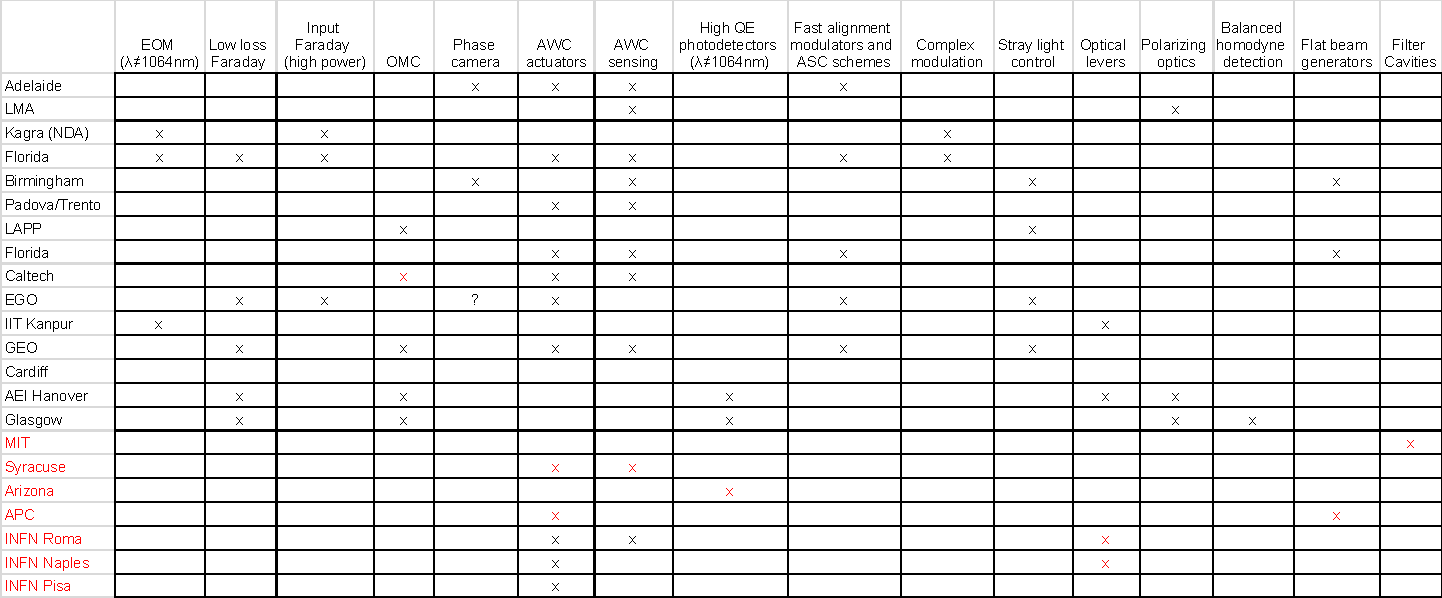
\includegraphics[scale=0.65]{Figures/auxopticssurvey.pdf}
\caption{The current status of global gravitational wave detector auxiliary optics R\&D, based on the responses to an email survey and the knowledge of subcommittee members.}\label{figauxopticsssurvey}
\end{figure}

The remainder of this section is subdivided into a discussion of the requirements for each auxiliary optics subcategory in the context of laser wavelengths between 1 and 1.55\,$\mu$m and 1.55\,$\mu$m and above. Where there is expected to be no major difference between the R\&D required for both wavelength ranges, the R\&D will be described in the section for the shorter wavelength range only. 

\subsubsection{1-1.55\,$\mu$m laser wavelength R\&D requirements}
\paragraph{Input optics}
In that wavelength range, we do not expect particular issues with respect to the 2G. The main issue might concern scattered light management and beam jitter mitigation.
We mostly rely the developments which have been made for the first and second generation of GW detectors at 1.064 $\mu$m. For 1.55$\mu$m, there will be for sure the need of R\&D on wavelength dependent optical devices such as the Faraday isolator especially if we want to work at very high power at 1.55$\mu$m. Some R\&D activities are already planned in several groups (IAP, UF and EGO) so we do not expect major issues on that point.
Below we just list the most important sub-parts of the IO.
\begin{itemize}
\item	High power Faraday isolator for 1 and 1.55 um R\&D on-going.
\item	EOMs. Seems to be under control but might be needed to think about RAM noise.
\item	Complex modulation - can be used to minimize am (better control of locking point offsets). R\&D ongoing.
\item	Fast alignment actuators. Alignment sensing and/or control. R\&D ongoing.
\item	Flat beam generators (LG modes etc.). Not much active research recently.
\item	Input mode cleaner and frequency stabilization scheme (not R\&D more related to design choices). 
\end{itemize}
\paragraph{Output optics}
The main point will consist in mitigating the scattered light which is harmful for the Interferometer sensitivities in the second generation of GW detector.
R\&D activity on OMC could be useful?
For what concerns the development of low-loss Faraday isolator for the squeezed light injection at 1$\mu$m, the situation seems well under control. A few groups are working on that topic (UF,AEI and EGO). Some good results have been obtained recently with the demonstration of sub percent loss Faraday isolators (see for example refLLFI). We can reasonably expect to get below 0.5\% for a single pass. If the losses have to be lower some particular effort will have to be devoted to that topic.\\ 
Filter cavity

refLLFI E. Genin and G. Pillant, Development of Low loss Faraday isolators at EGO, Presentation at LVC Sonoma meeting, March 2018, \url{https://dcc.ligo.org/DocDB/0150/G1800468/001/LowlossFIupdate_20032018_v2.pdf}

\paragraph{Active wavefront control}
At 1um we can base the TCS system on what has been used in the second generation GW detectors.
At 1.55$\mu$m, it could be required to change the actuation techniques if we change the test mass material. 
In general we expect that the requirements on mode matching and contrast defect become significantly more stringent for upgrades to the Advanced detectors, and for the 3G detectors. This is primarily because of the expected addition of squeezed light enhanced to the detectors. Mode mismatches in the core interferometer and the signal extraction chain can cause at best a reduction in the benefit of squeezing at certain frequencies (i.e. in the case of mode mismatch to a filter cavity), and at worst an effective optical loss 

\paragraph{Stray light mitigation}
The light absorption from the baffles is very dependent on the wavelength. So it is likely that what will work at 1um but not at 1.55 $\mu$m. R\&D will be required to find new materials suitable for 1.55$\mu$m.  

\paragraph{Other auxiliary optics}
{\bf Optical levers}
Increasing the length of the arm cavities can represent a problem from the optical levers point of view. A preliminary study should be done in order to understand the requirements on the suspended optics residual motion tolerated to be able to lock the arm cavities (40 km is quite long!).

{\bf Alignment sensing schemes}

{\bf Polarization optics}
In the case that a Sagnac-type interferometer is to be used for 3G detectors, one option will be a polarization based Sagnac

\subsubsection{1.55+\,$\mu$m laser wavelength R\&D requirements}
Above 1.55 $\mu$m and especially if we go to 2 or 2.1 $\mu$m things are new and it is sure exploratory activities will be required. Consider that now most in the laboratories involved in the business are equipped with optics laser sources and detectors for 1 $\mu$m wavelength. Going to 2 $\mu$m will require a huge funding effort form the agencies.\\

\paragraph{Input optics}

The most critical components remain the one which are wavelength dependent such as the Faraday isolator in particular.  Some R\&D activities are already planned in several groups (IAP, UF and EGO) to develop a high power vacuum compatible Faraday isolator for 2 $\mu$m.
At 2$\mu$m, Faraday isolators already exist (refEoT) but a high power vacuum compatible one will have to be developed since it cannot be found on the market. In that case, iron garnets should be considered as potential candidates. It could be Yttrium Iron Garnet (YIG) or bismuth-substituted iron garnet. Those materials have the advantage that the Faraday rotation effect is one order of magnitude larger than that of TGG in the near infrared region. This could help reducing the magnet size and the overall weight of the device.\\

refEoT EoT Makros series, \url{https://www.eotech.com/cart/3/faraday-rotators/makros-series-1900-2100nm-high-power-faraday-rotators}\\

Regarding the Electro optic modulation system, according to what we know Rubidium Titanyl Phosphate could be kept as EO crystal since it is also transparent on a wide wavelength range (0.5$\mu$m to 3.5$\mu$m) but some tests will have to be made in order to evaluate the absorption of this crystal at 2 $\mu$m which could represent an issue if high.

\paragraph{Output optics}
\paragraph{Active wavefront control}
\paragraph{Stray light mitigation}
\paragraph{Other auxiliary optics}

% \subsubsection{3G initial}
% \subsubsection{future}
\subsection{Pathways, required facilities, collaborations and mechanisms}

\subsubsection{Pathways and required facilities}
Many of the auxiliary optics subsystems can be developed in small laboratories in tabletop demonstrations. Filter cavities will be tested first in A+. 

\subsubsection{Type of collaboration required:  small/large}
\begin{itemize}
\item Collaborations between groups working on the different AO topics identified. 
\item Collaborations between AO and other subtopics (e.g. facilities, light sources, quantum noise etc.)
\end{itemize}
\subsubsection{Suggested mechanisms}

\subsection{Impact/relation to 2G and upgrades}
\paragraph{Input optics}


\paragraph{Output optics}
Filter cavities are being planned for installation at the Advanced LIGO and Advanced Virgo detectors as part of the A+ upgrade for Ligo and AdV+ upgrade for Virgo. We expect that some type of frequency dependent squeezing enhancement will be included in all 3G detectors, so the inclusion in the 2nd generation upgrades is of course beneficial in terms of preparatory R\&D.

\paragraph{Active wavefront control}
\paragraph{Stray light mitigation}
\paragraph{Other auxiliary optics}